\documentclass[tikz,border=10pt]{standalone}
\usetikzlibrary{shapes, arrows.meta, positioning, fit, calc}
\usetikzlibrary{arrows}
\tikzstyle{every task} = []
\tikzstyle{every gateway} = []
\tikzstyle{every sequence} = []
\tikzstyle{every message} = []
\tikzstyle{every association} = []
\tikzstyle{every event} = []

\tikzstyle{task} = [rectangle, draw, black,
                      minimum width=4em, minimum height=2em,rounded corners,align=center,every task]

\tikzstyle{gateway} = [diamond, draw, black,inner sep=0pt,minimum width=1em, minimum height=1em,every gateway]
\tikzstyle{sequence} = [->,>=triangle 45,every sequence]
\tikzstyle{message} = [o->,dashed,>=open triangle 45,every sequence]
\tikzstyle{association} = [->,densely dotted,>=angle 45,every association]
\tikzstyle{event} = [circle,minimum width=1.5em, minimum height=1.5em,draw,every event]
\tikzstyle{end event} = [event,ultra thick,every event]
\tikzstyle{intermediate event} = [event,double,every event]

\begin{document}

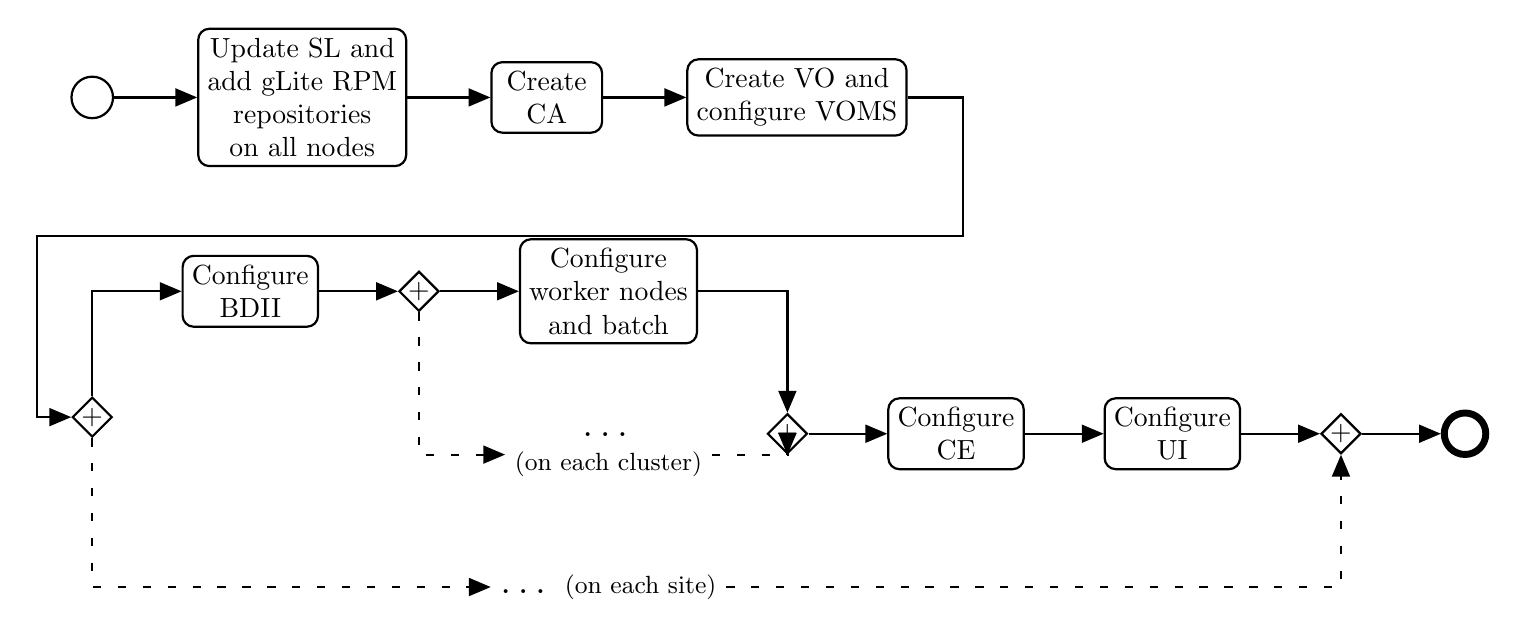
\begin{tikzpicture}[
roundnode/.style={circle, draw=black!60, fill=white!5, very thick, double, minimum size=7mm},
squarednode/.style={rectangle, draw=red!60, fill=red!5, very thick, minimum size=5mm},
]
%Nodes
% \node[squarednode]      (maintopic)                              {2};
% \node[roundnode]        (uppercircle)       [above=of maintopic] {$x_1$};
% \node[squarednode]      (rightsquare)       [right=of maintopic] {3};
% \node[roundnode]        (lowercircle)       [below=of maintopic] {4};
%
% %Lines
% \draw[->] (uppercircle.south) -- (maintopic.north);
% \draw[->] (maintopic.east) -- (rightsquare.west);
% \draw[->] (rightsquare.south) .. controls +(down:7mm) and +(right:7mm) .. (lowercircle.east);

  \tikzstyle{every task} = [thick,fill=white]
  \tikzstyle{every sequence} = [thick]
  \tikzstyle{every gateway} = [thick,fill=white]
  \tikzstyle{every event} = [thick,fill=white]
  \tikzstyle{end event} = [event,line width=2.5pt,fill=white]
  \node[event] (start) {};
  \node[task,node distance=3em,right=of start] (updglite) { Update SL and \\ add gLite RPM \\ repositories \\ on all nodes };
  \draw[sequence,->] (start) -- (updglite);
  \node[task,node distance=3em,right=of updglite] (ca) { Create \\ CA };
  \draw[sequence,->] (updglite) -- (ca);
  \node[task,node distance=3em,right=of ca] (vo) { Create VO and \\configure VOMS};
  \draw[sequence,->] (ca) -- (vo);
  \node[gateway,node distance=10em,below=of start] (pg) {+};

  \draw[sequence,->] (vo) -- ++(6em,0) -- ++(0,-5em) node(foo){} -- (pg |- foo) -- ++(-2em,0) node(foo2){} -- (foo2 |- pg) -- (pg);

  \node[task,above right=of pg] (bdii) {Configure \\ BDII};
  \draw[sequence,->] (pg) |- (bdii);
  \node[gateway,right=of bdii] (pg2) {+};
  \draw[sequence,->] (bdii) -- (pg2);
  \node[task,right=of pg2] (wn) {Configure \\ worker nodes\\ and batch};
  \draw[sequence,->] (pg2) -- (wn);
  \node[align=center,below=of wn] (etc2) { {\Large \ldots } \\ \small (on each cluster)};
  \draw[sequence,->,loosely dashed] (pg2) |- (etc2);
  \node[gateway,below right=of wn] (pg3) {+};
  \draw[sequence,->,loosely dashed] (etc2) -| (pg3);
  \draw[sequence,->] (wn) -| (pg3);
  \node[task,right=of pg3] (ce) {Configure \\ CE};
  \draw[sequence,->] (pg3) -- (ce);
  \node[task,right=of ce] (ui) {Configure \\ UI};
  \draw[sequence,->] (ce) -- (ui);
  \node[gateway,right=of ui] (pg4) {+};
  \draw[sequence,->] (ui) -- (pg4);
  \node[end event,right=of pg4] (end) {};
  \draw[sequence,->] (pg4) -- (end);
  \node[align=center,below=of etc2] (etc1) { {\Large \ldots } \small (on each site)};
  \draw[sequence,->,loosely dashed] (pg) |- (etc1);
  \draw[sequence,->,loosely dashed] (etc1) -| (pg4);
\end{tikzpicture}

\end{document}
